\begin{figure}
  \centering

  \small

  \newcommand{\w}[1]{\textcolor{white}{#1}}
  \def\svgwidth{0.9\textwidth}

  % INKSCAPE
%% Creator: Inkscape inkscape 0.92.2, www.inkscape.org
%% PDF/EPS/PS + LaTeX output extension by Johan Engelen, 2010
%% Accompanies image file 'vape_all.eps' (pdf, eps, ps)
%%
%% To include the image in your LaTeX document, write
%%   \input{<filename>.pdf_tex}
%%  instead of
%%   \includegraphics{<filename>.pdf}
%% To scale the image, write
%%   \def\svgwidth{<desired width>}
%%   \input{<filename>.pdf_tex}
%%  instead of
%%   \includegraphics[width=<desired width>]{<filename>.pdf}
%%
%% Images with a different path to the parent latex file can
%% be accessed with the `import' package (which may need to be
%% installed) using
%%   \usepackage{import}
%% in the preamble, and then including the image with
%%   \import{<path to file>}{<filename>.pdf_tex}
%% Alternatively, one can specify
%%   \graphicspath{{<path to file>/}}
%% 
%% For more information, please see info/svg-inkscape on CTAN:
%%   http://tug.ctan.org/tex-archive/info/svg-inkscape
%%
\begingroup%
  \makeatletter%
  \providecommand\color[2][]{%
    \errmessage{(Inkscape) Color is used for the text in Inkscape, but the package 'color.sty' is not loaded}%
    \renewcommand\color[2][]{}%
  }%
  \providecommand\transparent[1]{%
    \errmessage{(Inkscape) Transparency is used (non-zero) for the text in Inkscape, but the package 'transparent.sty' is not loaded}%
    \renewcommand\transparent[1]{}%
  }%
  \providecommand\rotatebox[2]{#2}%
  \newcommand*\fsize{\dimexpr\f@size pt\relax}%
  \newcommand*\lineheight[1]{\fontsize{\fsize}{#1\fsize}\selectfont}%
  \ifx\svgwidth\undefined%
    \setlength{\unitlength}{842.29600432bp}%
    \ifx\svgscale\undefined%
      \relax%
    \else%
      \setlength{\unitlength}{\unitlength * \real{\svgscale}}%
    \fi%
  \else%
    \setlength{\unitlength}{\svgwidth}%
  \fi%
  \global\let\svgwidth\undefined%
  \global\let\svgscale\undefined%
  \makeatother%
  \begin{picture}(1,0.70675867)%
    \lineheight{1}%
    \setlength\tabcolsep{0pt}%
    \put(0,0){\includegraphics[width=\unitlength]{vape_all.eps}}%
    \put(0.1193648,0.32835986){\color[rgb]{0,0,0}\makebox(0,0)[t]{\lineheight{0}\smash{\begin{tabular}[t]{c}$\mu_{i-1}$\end{tabular}}}}%
    \put(0.19549212,0.32835986){\color[rgb]{1,1,1}\makebox(0,0)[t]{\lineheight{0}\smash{\begin{tabular}[t]{c} \end{tabular}}}}%
    \put(0.12182045,0.56037307){\color[rgb]{0,0,0}\makebox(0,0)[t]{\lineheight{0}\smash{\begin{tabular}[t]{c}\w{$\pi_{i-1}$}\end{tabular}}}}%
    \put(0.47371048,0.32835986){\color[rgb]{0,0,0}\makebox(0,0)[t]{\lineheight{0}\smash{\begin{tabular}[t]{c}$\mu_i$\end{tabular}}}}%
    \put(0.82832099,0.32835986){\color[rgb]{0,0,0}\makebox(0,0)[t]{\lineheight{0}\smash{\begin{tabular}[t]{c}$\mu_{i+1}$\end{tabular}}}}%
    \put(0.47703537,0.56037307){\color[rgb]{0,0,0}\makebox(0,0)[t]{\lineheight{0}\smash{\begin{tabular}[t]{c}\w{$\pi_i$}\end{tabular}}}}%
    \put(0.83014525,0.56037307){\color[rgb]{0,0,0}\makebox(0,0)[t]{\lineheight{0}\smash{\begin{tabular}[t]{c}\w{$\pi_{i+1}$}\end{tabular}}}}%
    \put(0.0957776,0.0813595){\color[rgb]{0,0,0}\makebox(0,0)[t]{\lineheight{0}\smash{\begin{tabular}[t]{c} \end{tabular}}}}%
    \put(0.19867469,0.34932631){\color[rgb]{1,1,1}\makebox(0,0)[t]{\lineheight{0}\smash{\begin{tabular}[t]{c}\w{$\delta_{i-1}$}\end{tabular}}}}%
    \put(0.55190142,0.34913153){\color[rgb]{1,1,1}\makebox(0,0)[t]{\lineheight{0}\smash{\begin{tabular}[t]{c}\w{$\delta_i$}\end{tabular}}}}%
    \put(0.90678583,0.34939367){\color[rgb]{1,1,1}\makebox(0,0)[t]{\lineheight{0}\smash{\begin{tabular}[t]{c}\w{$\delta_{i+1}$}\end{tabular}}}}%
    \put(0.19724716,0.03888422){\color[rgb]{0,0,0}\makebox(0,0)[t]{\lineheight{0}\smash{\begin{tabular}[t]{c}$\hat{\mu}_{i-1}$\end{tabular}}}}%
    \put(0.55436625,0.03888422){\color[rgb]{0,0,0}\makebox(0,0)[t]{\lineheight{0}\smash{\begin{tabular}[t]{c}$\hat{\mu}_i$\end{tabular}}}}%
    \put(0.9052044,0.03888422){\color[rgb]{0,0,0}\makebox(0,0)[t]{\lineheight{0}\smash{\begin{tabular}[t]{c}$\hat{\mu}_{i+1}$\end{tabular}}}}%
    \put(0.98458269,0.49312545){\color[rgb]{0,0,0}\makebox(0,0)[rt]{\lineheight{0}\smash{\begin{tabular}[t]{r}\w{$\hat{\pi}_{i+1}$}\end{tabular}}}}%
    \put(0.24528255,0.4931251){\color[rgb]{0,0,0}\makebox(0,0)[t]{\lineheight{0}\smash{\begin{tabular}[t]{c}\w{$\hat{\pi}_{i-1}$}\end{tabular}}}}%
    \put(0.60324557,0.4931251){\color[rgb]{0,0,0}\makebox(0,0)[t]{\lineheight{0}\smash{\begin{tabular}[t]{c}\w{$\hat{\pi}_i$}\end{tabular}}}}%
    \put(0.1206534,0.06544562){\color[rgb]{0,0,0}\makebox(0,0)[t]{\lineheight{0}\smash{\begin{tabular}[t]{c}$\mu_{i-1}$\end{tabular}}}}%
    \put(0.4749991,0.06544562){\color[rgb]{0,0,0}\makebox(0,0)[t]{\lineheight{0}\smash{\begin{tabular}[t]{c}$\mu_i$\end{tabular}}}}%
    \put(0.82960961,0.06544562){\color[rgb]{0,0,0}\makebox(0,0)[t]{\lineheight{0}\smash{\begin{tabular}[t]{c}$\mu_{i+1}$\end{tabular}}}}%
    \put(0.01194257,0.65915071){\color[rgb]{0,0,0}\makebox(0,0)[lt]{\lineheight{0}\smash{\begin{tabular}[t]{l}1\end{tabular}}}}%
    \put(0.01160093,0.57261339){\color[rgb]{0,0,0}\makebox(0,0)[lt]{\lineheight{0}\smash{\begin{tabular}[t]{l}2\end{tabular}}}}%
    \put(0.00653804,0.49568081){\color[rgb]{0,0,0}\makebox(0,0)[lt]{\lineheight{0}\smash{\begin{tabular}[t]{l}3\textsf{A}\end{tabular}}}}%
    \put(0.00653845,0.34751437){\color[rgb]{0,0,0}\makebox(0,0)[lt]{\lineheight{0}\smash{\begin{tabular}[t]{l}3\textsf{B}\end{tabular}}}}%
    \put(0.0113686,0.21454449){\color[rgb]{0,0,0}\makebox(0,0)[lt]{\lineheight{0}\smash{\begin{tabular}[t]{l}4\end{tabular}}}}%
    \put(0.00651485,0.1385617){\color[rgb]{0,0,0}\makebox(0,0)[lt]{\lineheight{0}\smash{\begin{tabular}[t]{l}5\textsf{A}\end{tabular}}}}%
    \put(0.00651485,0.07872525){\color[rgb]{0,0,0}\makebox(0,0)[lt]{\lineheight{0}\smash{\begin{tabular}[t]{l}5\textsf{B}\end{tabular}}}}%
    \put(0.01169903,0.02743687){\color[rgb]{0,0,0}\makebox(0,0)[lt]{\lineheight{0}\smash{\begin{tabular}[t]{l}6\end{tabular}}}}%
    \put(0.21914871,0.60855135){\color[rgb]{0.62352941,0,0.52941176}\makebox(0,0)[t]{\lineheight{0}\smash{\begin{tabular}[t]{c}$\alpha_{i-1,i}^2$\end{tabular}}}}%
    \put(0.56974768,0.60855091){\color[rgb]{0.62352941,0,0.52941176}\makebox(0,0)[lt]{\lineheight{0}\smash{\begin{tabular}[t]{l}$\alpha_{i,i+1}^2$\end{tabular}}}}%
    \put(0.36165505,0.50407502){\color[rgb]{0.62352941,0,0.52941176}\makebox(0,0)[t]{\lineheight{0}\smash{\begin{tabular}[t]{c}$\alpha_{i-1,i}^2$\end{tabular}}}}%
    \put(0.71415359,0.50502481){\color[rgb]{0.62352941,0,0.52941176}\makebox(0,0)[lt]{\lineheight{0}\smash{\begin{tabular}[t]{l}$\alpha_{i,i+1}^2$\end{tabular}}}}%
    \put(0.31438169,0.04152979){\color[rgb]{0,0.78431373,1}\makebox(0,0)[t]{\lineheight{0}\smash{\begin{tabular}[t]{c}$\alpha_{i-1,i}$\end{tabular}}}}%
    \put(0.66770166,0.04152979){\color[rgb]{0,0.78431373,1}\makebox(0,0)[t]{\lineheight{0}\smash{\begin{tabular}[t]{c}$\alpha_{i,i+1}$\end{tabular}}}}%
    \put(0.32522196,0.54664964){\color[rgb]{1,0.79607843,0.0745098}\makebox(0,0)[t]{\lineheight{0}\smash{\begin{tabular}[t]{c}$\omega_{i-1}$\end{tabular}}}}%
    \put(0.68128491,0.54664964){\color[rgb]{1,0.79607843,0.0745098}\makebox(0,0)[t]{\lineheight{0}\smash{\begin{tabular}[t]{c}$\omega_i$\end{tabular}}}}%
  \end{picture}%
\endgroup%

  \caption{Overview of possible layer-specific message passing in \textsf{VAPE} coupling. Assignment of nodes to layers is loosely based on Figure 3 in \cite{Shipp2016}}.
\end{figure}